\subsection{FPGA Bridges}
\label{sec:FPGA_bridge}
The {\it FPGA bridges} depicted in Figure~\ref{fig:block_diagram} provide connections between
the HPS and FPGA in the Cyclone V SoC device. The bridges are enabled, or disabled, 
by using the {\it Bridge reset} register, which is illustrated in 
Figure~\ref{fig:FPGA_bridge} and has the address {\sf 0xFFD0501C}.  
Three distinct bridges exist, called {\it HPS-to-FPGA}, {\it lightweight HPS-to-FPGA}, and 
{\it FPGA-to-HPS}.  In the \systemName~the first two of these bridges are used to
connect the ARM A9 processor to the FPGA.  As indicated in 
Figure~\ref{fig:FPGA_bridge} the bridges are enabled/disabled by bits $0-2$ of the 
{\it Bridge reset} register.  To use the memory-mapped peripherals in the FPGA, software 
running on the ARM A9 must enable the HPS-to-FPGA and lightweight HPS-to-FPGA bridges by
setting bits \#0 and \#1 of the {\it Bridge reset} register to 0. 
We should note that if a user program is downloaded and run on the ARM A9 by using the
\productNameMed{}, described in Section~\ref{sec:monitor_program},
then these bridges are automatically enabled before the user program is started.

\begin{figure}[h!]
   \begin{center}
       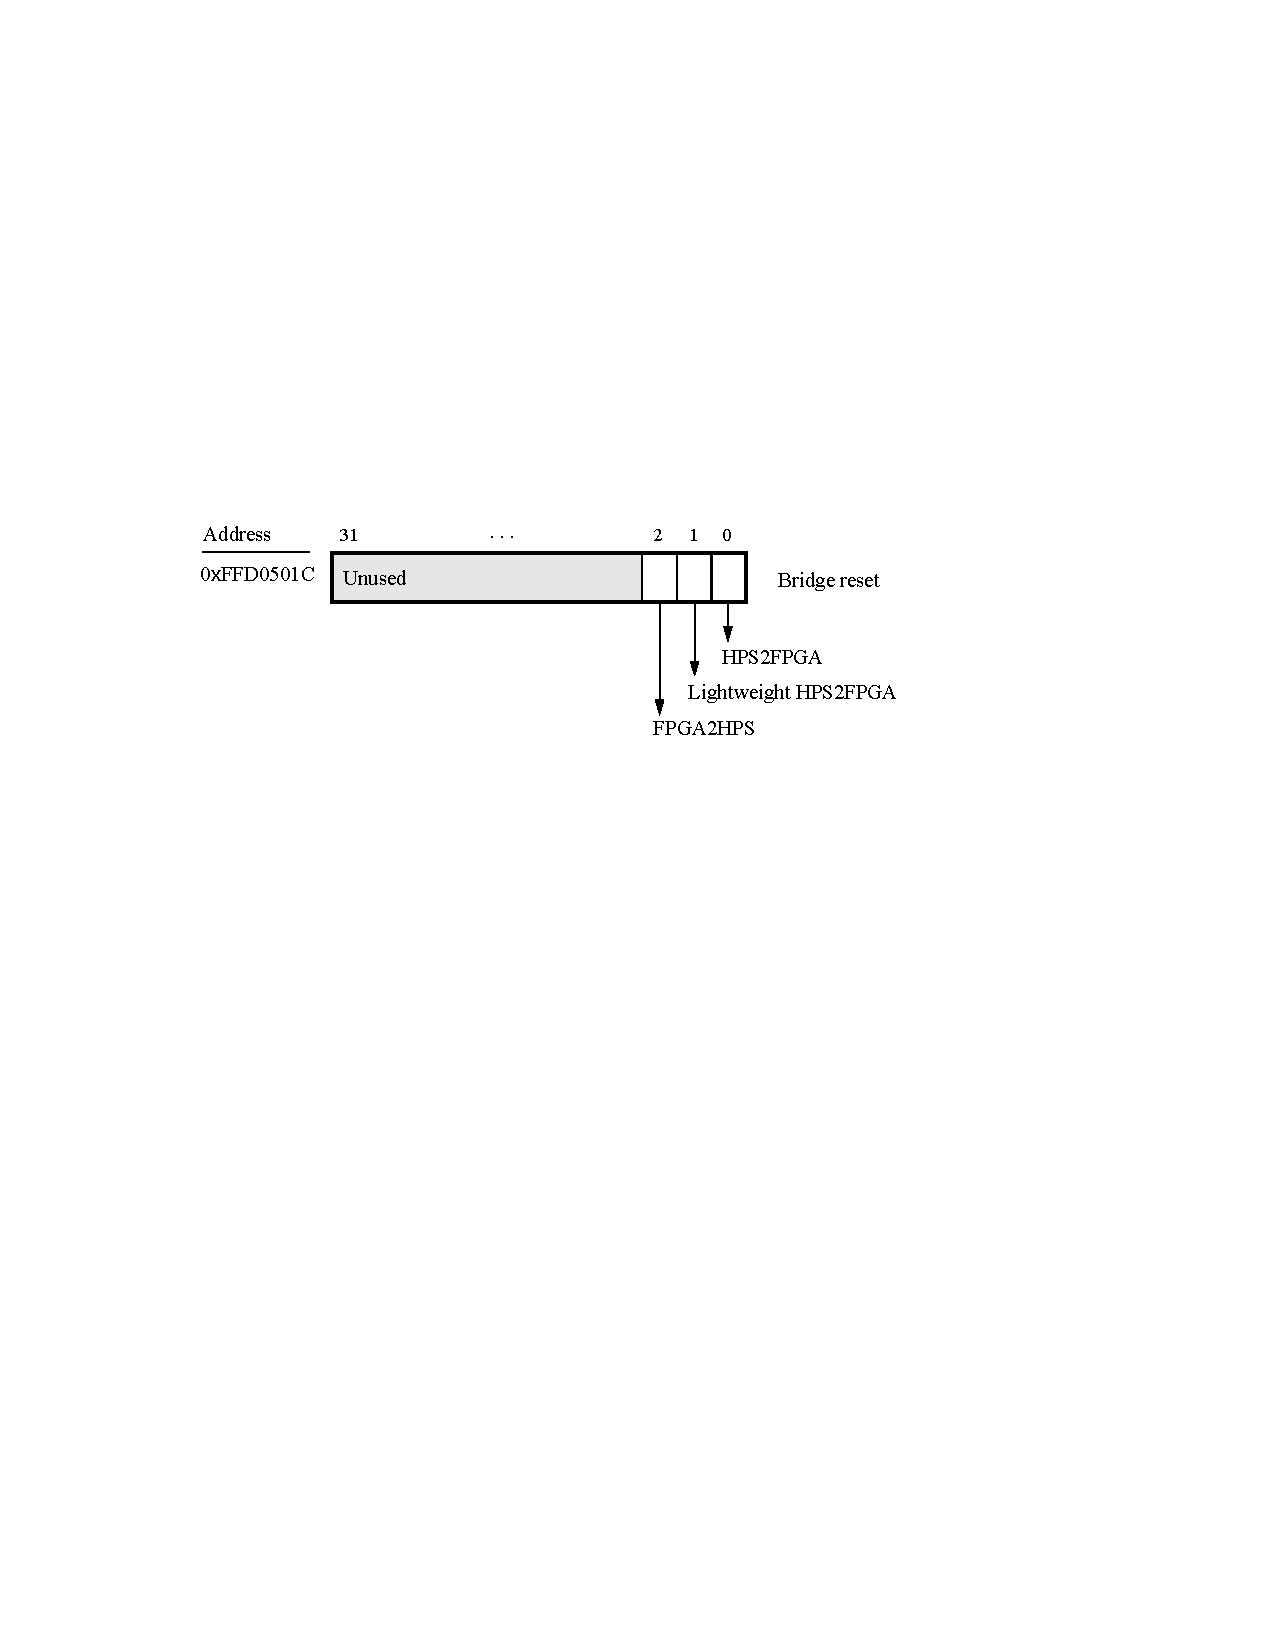
\includegraphics{../../../common/figs/HPS_FPGA_Bridges.pdf}
   \end{center}
   \caption{FPGA bridge reset register.}
	\label{fig:FPGA_bridge}
\end{figure}

In addition to the components described above, the HPS also provides a number of other
peripheral devices, such as USB, Ethernet, and a 3-D accelerometer (G-sensor). The
G-sensor is described in the tutorial {\it Using the Accelerometer on DE-series Boards}, 
which is available in the \texttt{Hardware Components} section of the
\href{https://www.fpgacademy.org/tutorials.html} {FPGAcademy.org} website.
Documentation about the other devices 
connected to the HPS can be found in the {\it Cyclone V Hard Processor System
Technical Reference Manual}, as well as in the {\it \DEBoard~Board User Manual}.


